\documentclass[../main]{subfiles}
\begin{document}
    \setcounter{secnumdepth}{2}
    \chapter{序論}
        \section{背景}
        近年,商業施設での清掃作業や屋外での宅配など,屋内外を問わず多くの場所で自律移動ロボットが活用されている.
        それらのロボットを安全かつ正確に運用するためには,自己位置推定をはじめとする様々な機能を持たせる必要がある.
        現在,商業施設などで用いられている自律移動ロボットは,あらかじめセンサにより取得した環境の詳細なデータを持つメトリックマップと呼ばれる
        地図を用いて自己位置推定を行なっている.しかし,詳細な地図を用いた自己位置推定は,事前に取得した地図中になかったものが環境中に置かれると
        自己位置推定に致命的な支障をきたすという問題がある.
        
        
        一方,人はそのような詳細な地図がなくても,「次の交差点で右」のような言葉の情報に基づき目的地まで移動することができる.
        そこで,そのような人の移動する能力をロボットの自律移動に応用する手法が研究されている.
        例えば,島田らは人の道案内に注目し,人の道案内のようにロボットを目的地まで移動させるナビゲーションの手法を提案した\cite{shimada_paper1}\cite{shimada_paper2}.
        この研究では,人が道案内で移動するには通路の特徴(形状)を重視しているということをアンケートにより収集し,
        ナビゲーションに用いるトポロジカルマップと呼ばれる地図と,シナリオと呼ばれる道案内を言葉に表現したものの形式を決め,
        実ロボットにより提案したナビゲーション手法の有効性を検証した.
        検証の結果,通路の特徴の認識が正しく行われた場合は提案したナビゲーション手法により目的地に到達できるが,
        誤認識が起きた場合はロボットが経路から外れ,ナビゲーションに失敗してしまうということが報告されている.
        また,この手法では通路の特徴の認識にLiDARを使用しており,誤認識は開いているドアや隙間にLiDARが反応したことが原因であると述べられている.
        そこで,通路の特徴認識にカメラ画像を用いることで誤認識を解消し,ナビゲーション途中に経路から外れるという問題を解決できるのではないかと考えた.

        \newpage

        \section{目的}
        本研究は,全天球カメラ画像に基づく通路の特徴認識の手法を提案する.そして,先行研究により提案された実ロボットを用いた
        トポロジカルマップとシナリオに基づくナビゲーションに対し,認識した通路の特徴情報を適用することで本手法の有効性を検証する.
        検証の際は,本研究と先行研究のナビゲーション結果に着目し,その成功回数を比較することとする.


        また,本研究では\fref{figure::image_exp}に示すような,全天球カメラの標準的なフォーマットである正距円筒図法という形式で画像を扱う.

        \begin{figure}[H]
            \centering
            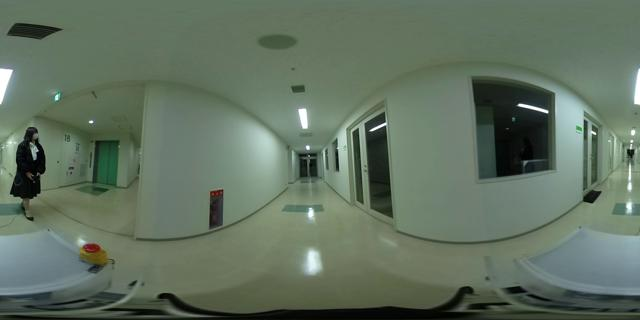
\includegraphics[width=10cm]{../images/18F_aisle_exp.jpg}
            \caption{Example of spherical camera image of equirectangular projection}
            \label{figure::image_exp}
        \end{figure}
        
        \newpage

        \section{関連研究}
        

        \section{本論文の構成}
        本論文ではまず,第1章で研究背景,目的,関連研究について述べた.第2章では,本研究で用いる要素技術について述べる.また,第3章では提案した手法について述べ,
        第4章では提案した手法の有効性の検証を行う.また,第5章では4章で行なった実験の結果をまとめ,考察を行う.最後に,第6章で本研究のまとめを行う.
\end{document}